%
% Homework Details
% - Title
% - Due date
% - University
% - Class
% - Class Alias
% - Class Section
% - Instructor
% - Author
% - AuthorID
%

\newcommand{\hmwkID}{1}
\newcommand{\hmwkTitle}{Final Project Report}
\newcommand{\hmwkTopic}{Game Playing with DQfD and DQN}
\newcommand{\hmwkUniversity}{NTU}
\newcommand{\hmwkClass}{Applied Deep Learning}
\newcommand{\hmwkClassAlias}{ADL}
\newcommand{\hmwkClassSection}{Fall 2017}
\newcommand{\hmwkClassInstructor}{Yun-Nung (Vivian) Chen and Hung-Yi Lee}
\newcommand{\hmwkTeam}{Praise The Sun}
\newcommand{\langver}{Trad. Chinese}



\documentclass{article}

%
% Packages
%

\usepackage{enumitem}
\usepackage{amsmath}
\usepackage{fancyhdr}
\usepackage{lastpage}
\usepackage{titlesec}
\usepackage[hidelinks]{hyperref}
\usepackage{cleveref}
\usepackage{listings}
\usepackage{bm}
\usepackage{float}
\usepackage{amsthm}
\usepackage{booktabs}

\usepackage{pgfplots}
\pgfplotsset{compat=1.7}
\usepackage{pgf,tikz}
\usepackage{mathrsfs}
\usetikzlibrary{arrows}
\usetikzlibrary[patterns]

\usepackage{xcolor}
\hypersetup{
    colorlinks,
    linkcolor={red!50!black},
    citecolor={blue!50!black},
    urlcolor={blue!80!black}
}

% additional packages
\usepackage{lettrine} % large initial
\usepackage{amsfonts} % mathbb

%
% Chinese
%

\usepackage{xeCJK}
\setCJKmainfont{Noto Sans CJK TC Regular}

\XeTeXlinebreaklocale "zh"
\XeTeXlinebreakskip = 0pt plus 1pt

%
% Basic Document Settings
%

\topmargin=-0.45in
\evensidemargin=0in
\oddsidemargin=0in
\textwidth=6.5in
\textheight=9.0in
\headsep=0.25in

\linespread{1.3}

% multirow
\usepackage{multirow}
\usepackage{multicol}
\usepackage{arydshln}
% figure name
\renewcommand{\figurename}{圖}
\renewcommand{\tablename}{表}

\makeatletter
\def\hlinewd#1{%
  \noalign{\ifnum0=`}\fi\hrule \@height #1 \futurelet
   \reserved@a\@xhline}
\makeatother

% fancy style

\pagestyle{fancy}
%\lhead{\hmwkTeam}
\lhead{\hmwkClass\ (\hmwkUniversity, \hmwkClassSection)}
%\chead{}
\rhead{\hmwkTeam: \hmwkTitle\ (\langver)}
%\rhead{\hmwkClass\ (\hmwkUniversity, \hmwkClassSection): \hmwkTitle (\langver)}
\cfoot{\thepage\ of \pageref{LastPage}}

%
% Title Page
%

%\title{
%  % \vspace{2in}
%  \textmd{\textbf{\hmwkClass:\ \hmwkTitle}}\\
%  \textmd{\textbf{\hmwkTopic}} \\
%  \vspace{0.1in}\large{\textit{Instructors \hmwkClassInstructor}}
%  % \vspace{3in}
%}

\title{
   \vspace{-1.5cm}
  \hmwkClass:\ \hmwkTitle\\
  \textbf{\hmwkTopic} \\
  \vspace{0.1in}\large{\textit{Instructors: \hmwkClassInstructor}}
   %\vspace{-1.5cm}
}

\author{
    \textit{Team: \textbf{\hmwkTeam}}
}
\date{}

\begin{document}

%\pagenumbering{gobble}
\maketitle
\thispagestyle{empty}
\thispagestyle{fancy}
% \pagebreak
\pagenumbering{arabic}

\lettrine[findent=1pt]{\fbox{深}}{ }度強化學習(Deep reinforcement learning)是利用既有的強化學習演算法,結合近年來表現很好的深度學習,所形成的一類機器學習模型,目前在許多領域,例如電腦對局、機器人學、以及機器玩遊戲等,已有很好甚至超越人類的成果。不過,根據先前作業的經驗,傳統的深度強化學習模型在訓練期間頗為耗時,而且就算使用相同環境訓練相同模型,其訓練的成效有時也好壞不一。為了解決這樣的問題,(T. Hester et al., 2017)\cite{DBLP:journals/corr/HesterVPLSPSDOA17} 提出了 DQfD (Deep Q-Learning from Demonstrations)模型,並說明該模型可以僅僅藉由少量的遊戲演示資料來加速模型的訓練。本報告將以數種Atari遊戲作為訓練環境,比較DQfD以及DQN(以及其變形)在這些遊戲中的學習狀態以及成果,並分析導致這些模型結果上差異的因素。

\section{深度強化學習簡介}
在強化學習中,一個模型裡存有一環境(environment)以及主體(agent),而主體的行為模式可視為一馬可夫決策過程(Markov desicion process,MDP)。MDP可以以一個五元組$(S,A,R(\cdot,\cdot),T(\cdot, \cdot, \cdot),\gamma)$表示。$S$代表著所有狀態(state)的集合;$A$為所有可能行動(action)的集合;$R(s,a)$為一獎勵函數(reward function)(即給定目前狀態$s$以及目前行動$a$,其獎勵為多少);$T(s,a,s')=P(s'|s,a)$為一轉換函數(transition function),並服從某一機率分佈;$\gamma$則為折減率(discount factor)。而主體在這個環境中,會根據某個策略函數$\pi(s)$來行動。\par
在強化學習中,最常見的模型根據主體的性質主要分為基於策略(policy-based)以及基於價值(value-based)的模型:前者主要為直接尋找一個策略函數$\pi$使得其盡量接近最佳策略(即$\pi \rightarrow \pi^*$);而後者則是給定一個價值函數($Q^\pi (s,a)$),該函數的目的即是估計出在目前狀態$s$下,若採取某行動$a$所能帶來的預期價值(expected value),而我們會希望該函數可以準確估計出各種狀況下的預期價值(即$Q^\pi (s,a) \rightarrow Q^* (s,a)$),在這情況下,主體的最佳策略即為$\pi^*(s) = \arg \underset{a \in A}\max\ Q^*(s,a)$。\par
Deep Q-Learning(DQN,直譯為「深度Q學習」)是一種常見的基於價值的深度強化學習模型。它的最佳價值函數可以以下面方程式(Bellman equation)表示:
\[Q^*(s,a) = \mathbb{E}\left[R(s,a) + \gamma \sum_{s'}P(s'|s,a) \underset{a'}\max\ Q^*(s',a')\right]\]
在DQN裡,我們會用一個深度學習網路來代表$Q^\pi$,而我們希望最後$Q^\pi$盡可能的接近$Q^*$。在實務上,我們會用平均平方錯誤(mean squared error, MSE)作為訓練時的誤差函數,且為了穩定訓練,還會固定目標項之參數,如下所示:
\[\mathcal{L}(w) = \mathbb{E}\left[\left(\underbrace{R(s,a) + \gamma \underset{a'}\max\ Q(s',a', w^-)}_{\text{target, update slowly}} - \underbrace{Q(s,a,w)}_{\text{online, update quickly}}\right)^2\right]\]
\par
其他常見的DQN模型還有:Double Q-Learning(DDQN)(H. van Hasselt et al., 2015)\cite{DBLP:journals/corr/HasseltGS15}以及Dueling Network (Z. Wang et al., 2015)\cite{DBLP:journals/corr/WangFL15}等。前者認為,利用目標網路(target network)選取未來預期最大價值的行動,容易有過度估計上的誤差(upward bias)。因此,該模型修正誤差函數成如下:
\[\mathcal{L}(w) = \mathbb{E}\left[\left(R(s,a) + \gamma Q(s',\underbrace{\arg \underset{a'}\max\ Q(s',a',w)}_{\text{online network chooses optimal } a'}, w^-) - Q(s,a,w)\right)^2\right]\],而後者則將網路修正成:
\[Q(s,a,w) = \underbrace{V(s,w)}_{\text{\emph{value}, action-independent}} + \underbrace{A(s,a,w)}_{\text{\emph{advantage}, action-dependent}}\]
基本概念為:有些狀態天生較好(無論行動為何,預期價值一定比較高),而有些則否,因此預期價值可以視為是目前狀態天生的預期價值(獨立於行動),加上在該狀態下,不同動作下所能提昇/減少的價值。

\section{DQfD:利用演示資料學習}
DQfD是一種混合了部份監督式學習(supervised learning)要素的強化學習演算法。相較於原始的DQN,DQfD在真正與環境互動訓練之前,會先使用一些事先收集好的演示資料(demonstration data)來進行預訓練(pre-training),之後才真正與環境互動進行強化。以真實的例子來比喻的話,這就有如一名運動員,先接受教練的訓練(專家演示)之後,才到比賽中(環境)累積經驗、強化自己的能力,而非直接在比賽中摸索。DQfD除了多了一個預訓練的過程,在誤差的計算上,也和原始的DQN頗有不同。首先,為了確保模型有去學演示資料的動作,所以加了以下(監督式學習的)誤差函數:
\[\mathcal{L}_E(w) = \underset{a \in A}\max [Q(s,a,w) + l(a_E, a)] - Q(s, a_E)\text{, where }l(a_E, a) = \left\{\begin{array}{cl}0 & \text{, if } a = a_E\\ k & \text{, otherwise and } k \text{ is a positive number}\end{array}\right.\],這樣強制任何其他動作之預期價值會至少比$a_E$還要少$k$,使得模型更傾向於去學演示資料的動作。除此之外,為了避免對於演示資料的過適(overfitting),對於網路的參數還會加一個L2-regularization loss($\mathcal{L}_{L2}(w)$)。最後,根據原始論文描述,為了讓模型符合原來的 Bellman equation,還會加上一個所謂的 n-step loss ($\mathcal{L}_n(w)$)。而總誤差為:
\[\mathcal{L}(w) = \underbrace{\mathcal{L}_{DQ}(w)}_{\text{original loss}} + \lambda_n \underbrace{\mathcal{L}_{n}(w)}_{\text{n-step loss}} + \lambda_E \underbrace{\mathcal{L}_{E}(w)}_{\text{supervised loss}} + \lambda_{L2} \underbrace{\mathcal{L}_{L2}(w)}_{\text{L2-regularization loss}}\]
\paragraph{額外設定} 除此之外,在預訓練完之後,如一般的DQN一樣,模型將會把過去走過的紀錄存進一個暫存的記憶體中(即 replay buffer)。一般而言,該記憶體大小是有限的,而在DQfD中,雖然演示資料(demonstration)和探索資料(exploration data)都是存在裡面然後被定期採樣出來,但是演示資料永遠不會被刪除,而舊的探索紀錄則會。此外,論文中亦建議使用prioritized replay buffer(T. Schaul et al., 2015) \cite{DBLP:journals/corr/SchaulQAS15}來讓演示資料有較高的優先權被採樣到。\par
因此,DQfD相較於DQN,總體上多了(一)演示資料(二)預訓練的過程(三)不同的誤差函數等設定。



\section{實驗設定}
在這次報告中,我們將沿用OpenAI的\texttt{gym}作為訓練環境,並且選了其中Atari遊戲中的三款(Seaquest, Enduro, SpaceInvader)作為實驗環境。而模型將會接受一經過預處理過的,最終大小為$4\times 84 \times 84$的灰階圖片(其中的4則為目前狀態往前算起的四張灰階圖片)。本次實驗將比較下列模型/設定:
\begin{itemize}
    \item 原始DQN(vanilla DQN)
    \item Double DQN
    \item Dueling DQN
    \item DQfD,使用n-step loss
    \item DQfD,不加n-step loss
\end{itemize}
在進行訓練之前,我們首先蒐集了一些人類玩家遊玩的資料。主要作法為將\texttt{gym}裡的動作控制改為由人類來操控,並且在遊玩過程中,自動紀錄每步之狀態、動作、獎勵、以及下次的狀態等。為了讓人類較有時間反應,亦降低了遊戲進行的速度。人類玩家為本組中的其中三名組員,各自玩其中一款遊戲,並各自蒐集了50000步以上的資料。

\begin{table}[]
\centering

%\label{my-label}
\resizebox{7cm}{!}{%
\begin{tabular}{lcccc}
\multicolumn{5}{c}{DQN Network}\\
\hlinewd{1.25pt}
type & activation & size & stride & output \\
\hline
 input & - & - & - & $4 \times 84 \times 84$ \\
 conv & ReLU & 8 & 4 & $32 \times 20 \times 20$ \\
 conv & ReLU & 4 & 2 & $64 \times 9 \times 9$ \\
 conv & ReLU & 3 & 1 & $64 \times 7 \times 7$ \\
 flatten & - & - & - & $3136$ \\
 linear & ReLU & - & - & $512$ \\
 linear & - & - & - & (\# of actions) \\
 output & - & - & - & (\# of actions) \\
\hlinewd{1.25pt}
\end{tabular}
}
\resizebox{7cm}{!}{%
\begin{tabular}{lccccc}
\multicolumn{6}{c}{Dueling DQN Network}\\
\hlinewd{1.25pt}
type & activation & size & stride & output & remarks \\
\hline
 input & - & - & - & $4 \times 84 \times 84$ &\\
 conv & ReLU & 8 & 4 & $32 \times 20 \times 20$ &\\
 conv & ReLU & 4 & 2 & $64 \times 9 \times 9$ &\\
 conv & ReLU & 3 & 1 & $64 \times 7 \times 7$ &\\
 flatten & - & - & - & $3136$ & F\\
\hdashline
\multicolumn{6}{c}{(value network)}\\
 linear & ReLU & - & - & $512$ & input: F\\
 linear & - & - & - & 1 &\\
 expand & - & - & - & (\# of actions) & V\\
\hdashline
\multicolumn{6}{c}{(advantage network)}\\
 linear & ReLU & - & - & $512$ & input: F\\
 linear & - & - & - & (\# of actions) &\\
 zero-mean & - & - & - & (\# of actions) & A\\
\hdashline
 add & - & - & - & (\# of actions) & V + A\\
 output & - & - & - & (\# of actions) &\\
\hlinewd{1.25pt}
\end{tabular}
}
\caption{DQN及Dueling Network 網路架構表,其中右圖中的value network以及advantage network是將flatten出來的結果作為輸入,而value network的輸出會複製成與advantage network維度相同的向量;advantage network的輸出則會將其分佈從$(\mu$, $\sigma^2)$標準化成$(0, \sigma^2)$,以避免value network無效。}
\label{tab:dqn}
\end{table}
表~\ref{tab:dqn} 為這次之網路架構圖,除了Dueling DQN 以外皆使用左側的架構,而我們在\texttt{pytorch 0.3.0}上實作上述網路。optimizer為RMSProp,學習速率(learning rate)為0.0001,折減率$\gamma$為0.99,目標網路、訓練網路之更新頻率分別為每1000步一次以及每4步一次,replay buffer 大小為10000,每次計算誤差時,從replay buffer 取樣出32筆資料。\par
DQfD中,首先會先預訓練350000次,取樣出演示資料的機率固定為0.3,n-step loss的n為10,若使用n-step loss時$\lambda_n$為1,$\lambda_E$為1,$l(a_E,a)$中的k為0.8。

\section{實驗結果與討論}

圖~\ref{fig:results} 為各模型在不同遊戲上之學習曲線。很明顯的可以看見DQfD之表現未如預期。我們大概分析了導致無法超越DDQN等演算法的可能原因:
\begin{itemize}
    \item 相較於原始論文的敘述,我們對記憶體中的資料做抽樣時,並未實作所謂的Priortized Replay Buffer,即未讓演示資料有較高的優先權被抽到,導致了模型比較不會學到專家示範的資料。
    \item 在預訓練完成時,模型應該就要能夠玩出一點分數,但我們的卻沒有。主要原因是因為實作DQfD時,我們所設定的隨機探索排程與其他模型一樣,從完全隨機遞減到5\%。這樣會導致預訓練的結果可能會被隨機探索洗掉。
    \item 我們的模型在加了 n-step loss 時結果有些異常,可能有其他實作上的缺陷。
\end{itemize}
綜合以上分析,我們這次在實作上稱不上是成功。未來若要在繼續深入探討,可能可以從上述的問題開始下手。


\begin{figure}

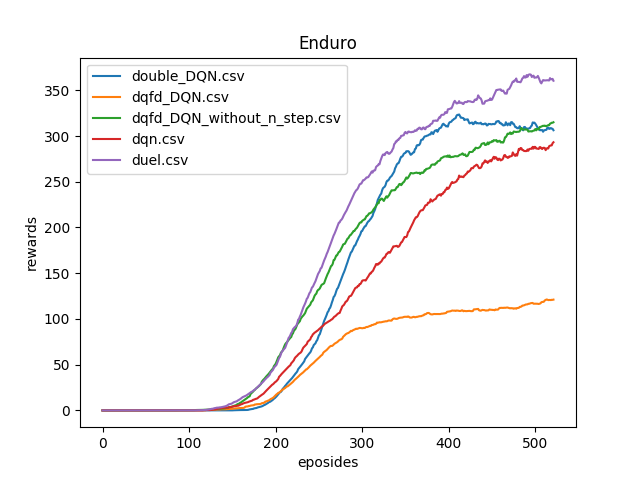
\includegraphics[scale=0.5]{../poster/figures/Enduro.png}
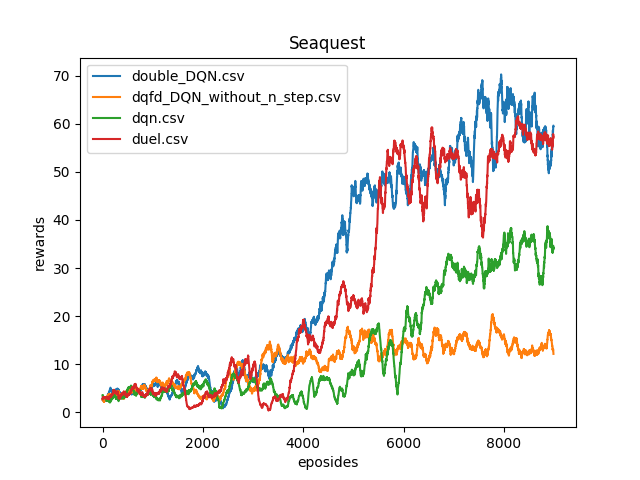
\includegraphics[scale=0.5]{../poster/figures/Seaquest.png}\\
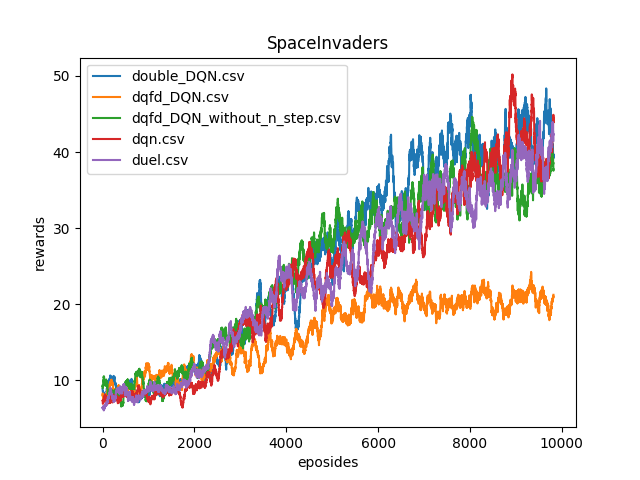
\includegraphics[scale=0.5]{../poster/figures/SpaceInvaders.png}

\caption{各模型之學習曲線。其中Enduro為一賽車遊戲,動作只有左、右、加速三種;而另外兩種比較偏向射擊遊戲,而Seaquest在複雜度上又比SpaceInvaders高。而DQfD之實作是以DDQN為基礎的,即其誤差函數中的$\mathcal{L}_{DQ}(w)$是與DDQN的相同。}
\label{fig:results}
\end{figure}




\renewcommand\refname{參考文獻}
\bibliographystyle{abbrv}
\bibliography{report}

\end{document}

